\documentclass[12pt]{article}
\usepackage{graphicx, amsmath}
\graphicspath{ {./} }
\setlength{\oddsidemargin}{0.25 in}
\setlength{\evensidemargin}{-0.25 in}
\setlength{\topmargin}{-0.6 in}
\setlength{\textwidth}{6.5 in}
\setlength{\textheight}{8.5 in}
\setlength{\headsep}{0.75 in}
\setlength{\parindent}{0 in}
\setlength{\parskip}{0.1 in}

\begin{document}
\thispagestyle{plain}
   \newpage
   \setcounter{page}{1}
   \noindent
   \begin{center}
   \framebox{
      \vbox{\vspace{2mm}
    \hbox to 6.28in { {\bf BioE 131: Intro to Computational Biology}
                        \hfill Fall 2020 }
       \vspace{4mm}
       \hbox to 6.28in { {\bf \Large \hfill Biological Databases and File Formats  \hfill} }
       \vspace{2mm}
       \hbox to 6.28in { {\it Professor: Ian Holmes \hfill} }
      \vspace{2mm}}
   }
   \end{center}
   {Notes written by Vikram Shivakumar}
   \vspace*{4mm}


\section{Introduction}

{\bf File formats} used in computational biology vary widely in structure and convention, and are often built for specific use cases by different communities with different needs. Some specific formats (like FASTA, GFF, BED, and SAM) are indicative of the these needs, representing specific types of data in uniform, flatfile-style formats. Other formats are more generic and extensible, applicable in multiple different contexts. These are also often used outside of computational biology (like XML and JSON), and follow specific schemas, or templates for how the data should look. \\[10pt]
{\bf Databases} are another method of storage for biological data. These repositories allow for adding, changing, retrieving, and deleting data, as well as user queries of select data. Often the databases impose a standardized form to avoid "dirty data", ensuring a level of quality and consistency across the repository. Databases can also be linked to other databases.

\subsection{Databases vs Files}

\textit{Why use databases at all? Why not just use files to store all data?}\\ One reason is that sometimes file formats can vary across filesystems, which can cause problems for data portability. Data validation also becomes more difficult with data stored in files. Also, linking and indexing data can be difficult across files in a filesystem.\\
\textit{Why not just use databases and no files?}\\
Lots of bioinformatics code and programs still use files to read and write data, and porting over to databases would be too difficult. Also, when running analyses of data, it is often quicker to start with files, and files are often easier to interpret and manually examine. 

\section{Databases}
\subsection{Relational vs non-Relational Databases}
{\bf Relational databases} store data that are related to each other in tables. Each table has multiple columns according to a {\bf schema}, which represent attributes of the data. These tables can be connected together by {\bf relational operators}, which specify links through keys. Accessing data from databases can become impossible to do manually as database size increases, but this can be achieved using the {\bf Structured Query Language (SQL)}. This language uses defined set operations to retrieve data from across tables in a database. Lastly, relational databases can be built and accessed through Relational Database Management Systems (RDBMS), like MySQL, Postgres, Oracle, etc.\\[10pt]
Databases like MongoDB, CouchDB, and MarkLogic are examples of non-relational databases. These databases follow the idea of "document store", using key-value pairs to point to data stored in documents. These systems can be faster and built larger, and can be useful in scenarios of big data and distributed data. 

\subsection{Properties of Databases}
Relational databases follow the {\bf ACID} properties (where an \textit{operation} is defined as viewing or modifying data):
\begin{enumerate}
    \item {\bf A}tomicity: operations are all-or-nothing
    \item {\bf C}onsistency: operations always leave a system in a valid state
    \item {\bf I}solation: operations do not affect each other and thus can be concurrent
    \item {\bf D}urability: operations are robust to system failures
\end{enumerate}
Another set of properties is {\bf CAP}:
\begin{enumerate}
    \item Consistency - each operation returns the most recent result
    \item Availability - each operation results in a response
    \item Partition-tolerance - operations still occur even if data is lost between partitioned nodes
\end{enumerate}
According to Brewer's theorem, a database cannot have all three of the CAP properties. For example, considering a network with two nodes (seperate partitions). If there is a failure between nodes (data cannot be sent between nodes), then either to preserve partition-tolerance, either responses to requests have to be halted (no availability), or possibly out-dated responses need to be sent (no consistency).

\section{File Formats}
Now let's take a look at a few different file formats that are commonly used in bioinformatics.
\subsection{FASTA and FASTQ}
{\bf FASTA} files are one of the most common filetypes in biology. They are used to store biological sequence data, for example DNA, RNA, or protein sequences. FASTA files are an example of a flatfile, and have a simple structure:
\begin{figure}[h!]
    \centering
    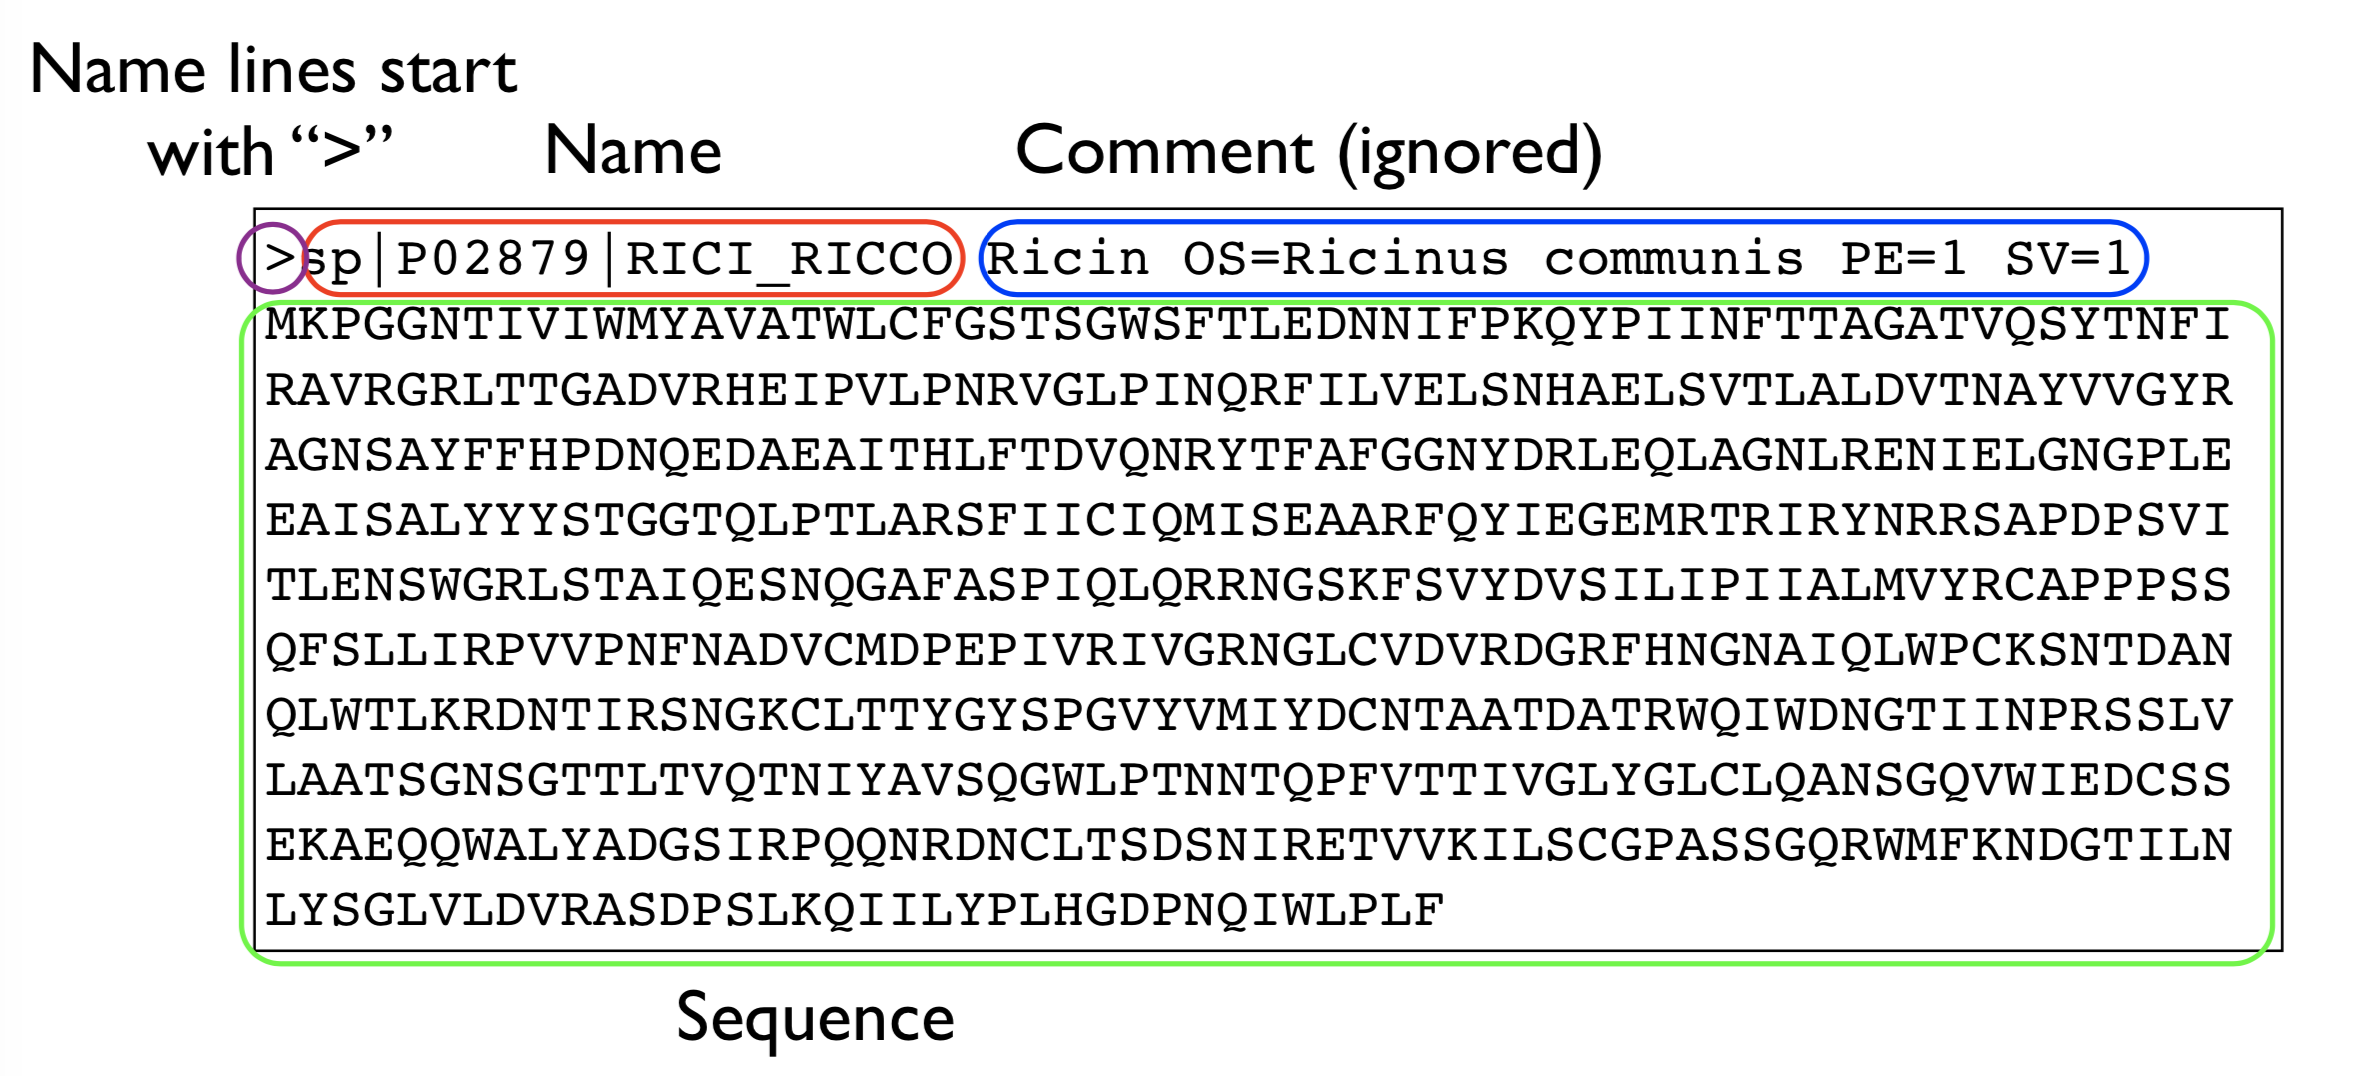
\includegraphics[width=.9\linewidth]{fasta}
    \caption{Example of a protein FASTA file}
    \label{fig:fasta}
\end{figure}

The sequence itself is written using the IUPAC single-letter codes for amino acids and nucleotides. This allows for degenerate codes, e.g. R=[AG],Y=[CT], N=[any nucleotide].\\[10pt]
{\bf FASTQ} files are similar to FASTA files in the representation of sequences, however it also includes an associated quality score for each base (or amino acid). To store this data, non-whitespace ASCII printable characters are used, e.g. “!” or “\%", each representing a quality score. Each sequence in a FASTQ file has exactly 4 lines: the name line (always starting with an ``@" symbol), the sequence itself, a line with only the character ``+", and the sequence of quality-score ASCII characters.\\[10pt]
\begin{figure}[h]
    \centering
    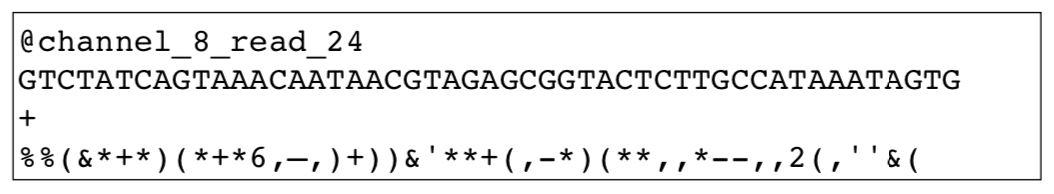
\includegraphics[width=.9\linewidth]{fastq}
    \caption{Example of sequencing read in FASTQ format}
    \label{fig:fastq}
\end{figure}
The quality scores in the FASTQ format are generally {\bf Phred quality scores}. These scores are related to the probability $P$ of a base-calling error during sequencing, and are calculated using the formula:
$$Q = -10\log_{10} P$$

\subsection{Annotation}
When working with sequence data, a common problem is identifying regions of significance, such as genes, splice sites, binding sites, or in the case protein sequences, protein domains and motifs. Naturally in these scenarios, a file format that is able to store \textbf{annotation} information for a sequence is crucial for many bioinformatics applications. \\[10pt]
One format that is commonly used for this purpose is the {\bf General Feature Format (GFF)}. GFF is a type of flatfile which specifies coordinates of various genomic features (such as exons, introns, promoters, etc.) for an accompanying sequence. A similar format, {\bf BED} lists sequence coordinates, but varies slightly in some conventions and formatting.\\[10pt]
One source of annotation and sequence data is {\bf Genbank}, a database of all publicly available DNA sequences (it is synced with other databases like EMBL and DDBJ). Large databases like these impose conventional forms on the annotation and sequence files to ensure standardization across the database, which in turn allows bioinformatics tools to work consistently with different datasets. {\bf Swiss-prot} and {\bf TrEMBL} are other examples of curated databases specifically for protein sequences. \\[10pt]
Another format for base-resolution annotation of sequences is the {\bf WIG (Wiggle)} format. This format allows for a numerical value to be associated with each base in the associated sequence, a form of quantitative annotation of sequence data. This is similar to the FASTQ format, where a value is associated which each base or amino acid in the sequence.
\subsection{Structure}
Biological sequences are presented in FASTA (or other formats) as linear strings of nucleotides or amino acids, but in biology, this is often not the case. Especially in the case of proteins and RNA, sequences tend to fold into complex structures, yet another piece of data that needs to be encoded into a file.\\[10pt]
The {\bf Protein Data Bank (PDB)} is a databank that stores 3D structures of large molecules like proteins, DNA, and RNA ({\it Note:} PDB is a databank, not a database, which means the data is not standardized or modified when submitted). Often the 3D structure is determined experimentally using techniques like x-ray crystallography, and submitted to the PDB. The \textbf{PDB filetype}, which is used to store this data, contains the atomic coordinates of these crystallographic structures in a column format. This filetype is relatively very old, and still resembles the structure of punch cards, which were once used to store the structural data. \\[10pt]
Another common structure to store is {\bf RNA secondary structure}. Due to base pairing within a single RNA sequence, these molecules often form various fold-back structures that need to be encoded in some way. The most common representation of this secondary structure is the {\bf dot-bracket notation}. This notation uses dots to represent unpaired bases, and paired brackets to represent base pairs across the sequence. These brackets can be nested to represent more complex structures like stem-loops. 
\begin{figure}[h]
    \centering
    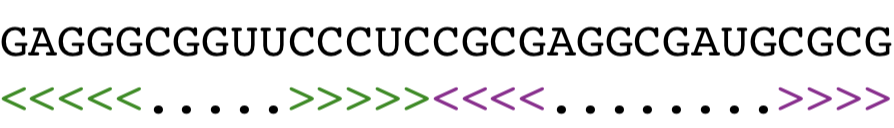
\includegraphics[width = .65\linewidth]{rna}  
    \caption{Example of dot-bracket notation for RNA structure}
    \label{fig:rna}
\end{figure}

However, one structure in particular cannot be represented using dot-bracket notation: {\bf pseudoknots}. These structures involve intercalated stem loops, which break the nested, paired nature of dot bracket notation.
\begin{figure}[h]
    \centering
    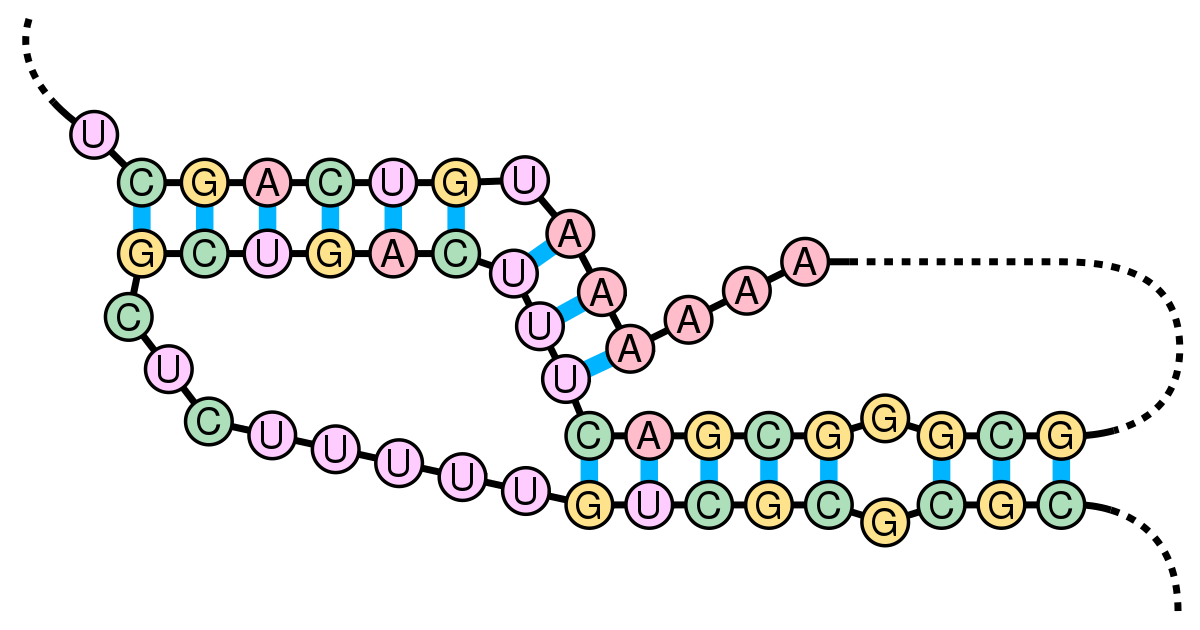
\includegraphics[width = .6\linewidth]{pseudo}
    \caption{Pseudoknot structure}
    \label{fig:my_label}
\end{figure}
\section{Alignment and Homology}
Another common task is determining how similar sequences are by aligning them to each other, and inferring evolutionary relationships from these alignments.
\subsection{Alignment}
Alignments can be stored in a straightforward way using a format we are already familiar with, FASTA files. Including multiple sequences from a {\bf Multiple Sequence Alignment (MSA)} in a single FASTA, and adding in gaps in each sequence to represent insertions or deletions, is a common way to store short alignments of sequences. However in some cases, there are more efficient methods of storing this data. \\[10pt]
Consider for example the task of aligning a million short ($\sim100$nt) reads (stored in a FASTQ file) to the human genome ($\sim3$ million bp). Using a gapped FASTA file would result in over a million sequences in a list, each with millions of gaps flanking the 100nt read sequence. This is extremely inefficient! The more common approach is to use a {\bf SAM} (or \textbf{BAM}) file. SAM files list each read and the alignment position in a reference sequence. That way, only the read sequences and a position need to be stored (assuming the reference is stored in a separate sequence file). A BAM file is the binary equivalent of the SAM file (and is often a smaller file size).\\[10pt]
SAM files use a method for efficiently storing alignments called the {\bf CIGAR} format. This format exploits the simple idea that base pairs that are identical to the reference do not need to be stored again. Thus each non-reference sequence is simply stored as a sequence of {\bf Matches (M)}, {\bf Insertions (I)}, or {\bf Deletions (D)} ({\it Note:} the distinction between an insertion and deletion is arbitrary and depends on which sequence is the ancestor of the other, which is often unknown). The CIGAR format is an example of \textbf{run-length encoding}, where multiple identical characters are encoded as a single variable with an associated count, a form of \textbf{lossless data compression}.
\begin{figure}[h]
    \centering
    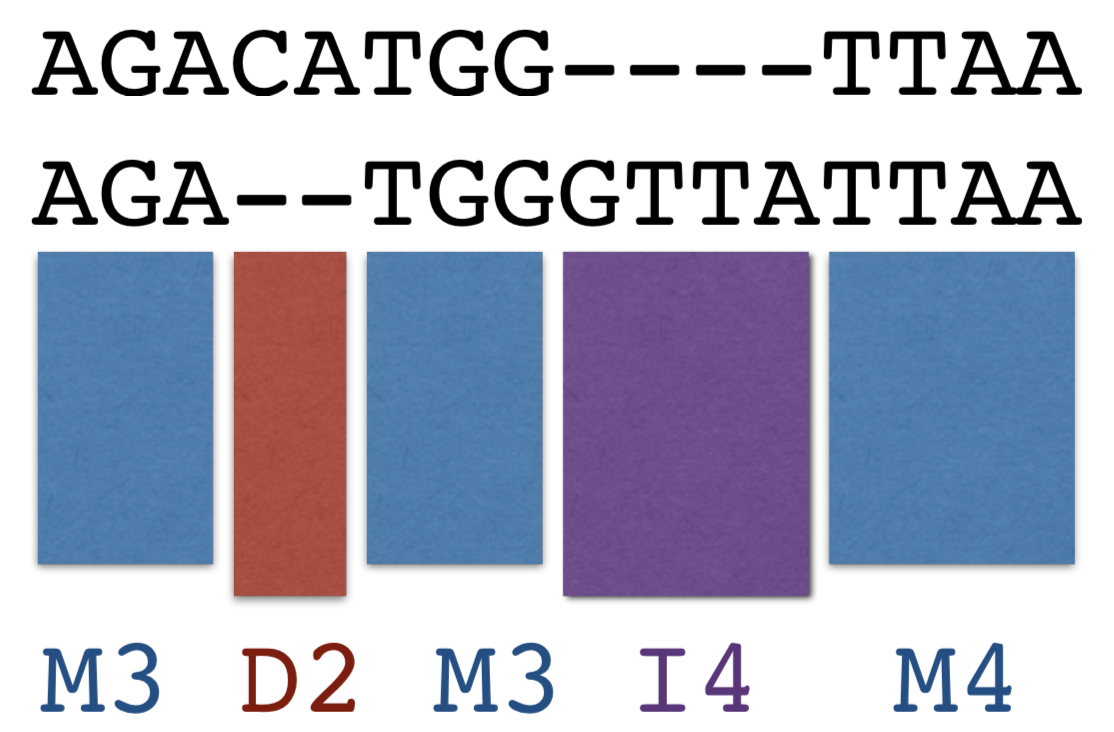
\includegraphics[height = .25\textheight]{cigar.png}
    \caption{Example of the CIGAR alignment format}
    \label{fig:cigar}
\end{figure}
\subsection{Evolutionary Homology}
Some databases like PFam, BLOCKS, COG, and PhyloFacts contain protein domain alignments. PFam and RFam in particular store alignments in the {\bf Stockholm format}. This format includes the sequence of each alignment entry along with other features of the alignment. Other databases like InterPro contain statistical profiles of protein domains, which can be used to characterize new protein sequences into domains and protein families.\\[10pt]
Lastly, another common type of data is the phyogeny, which stores the evolutionary relationships between species and sequences. Phylogenies naturally take the form of trees, which can be stored in a nested format. The {\bf New Hampshire (Newick) format} uses a nested structure to store the tree relationship between different items, along with information on branch lengths, statistical confidence values, etc. The NEXUS format is another format used to store phylogenies, is richer than Newick and contains more information on the sequence alignment and the taxa in the phylogeny.

\section{Parsers}
Each format has its own type of data, conventions, and standard form, which needs to be parsable in order to be useful in bioinformatic code. Many parser libraries exist in each programming language, so generally no manual parsing is needed. Depending on the format, some parsers may use models like {\bf finite state machines} or data structures like {\bf stacks} (for nested structures) to parse files into the relevant data types. The following is an example state machine to parse a FASTA file:
\begin{figure}[h]
    \centering
    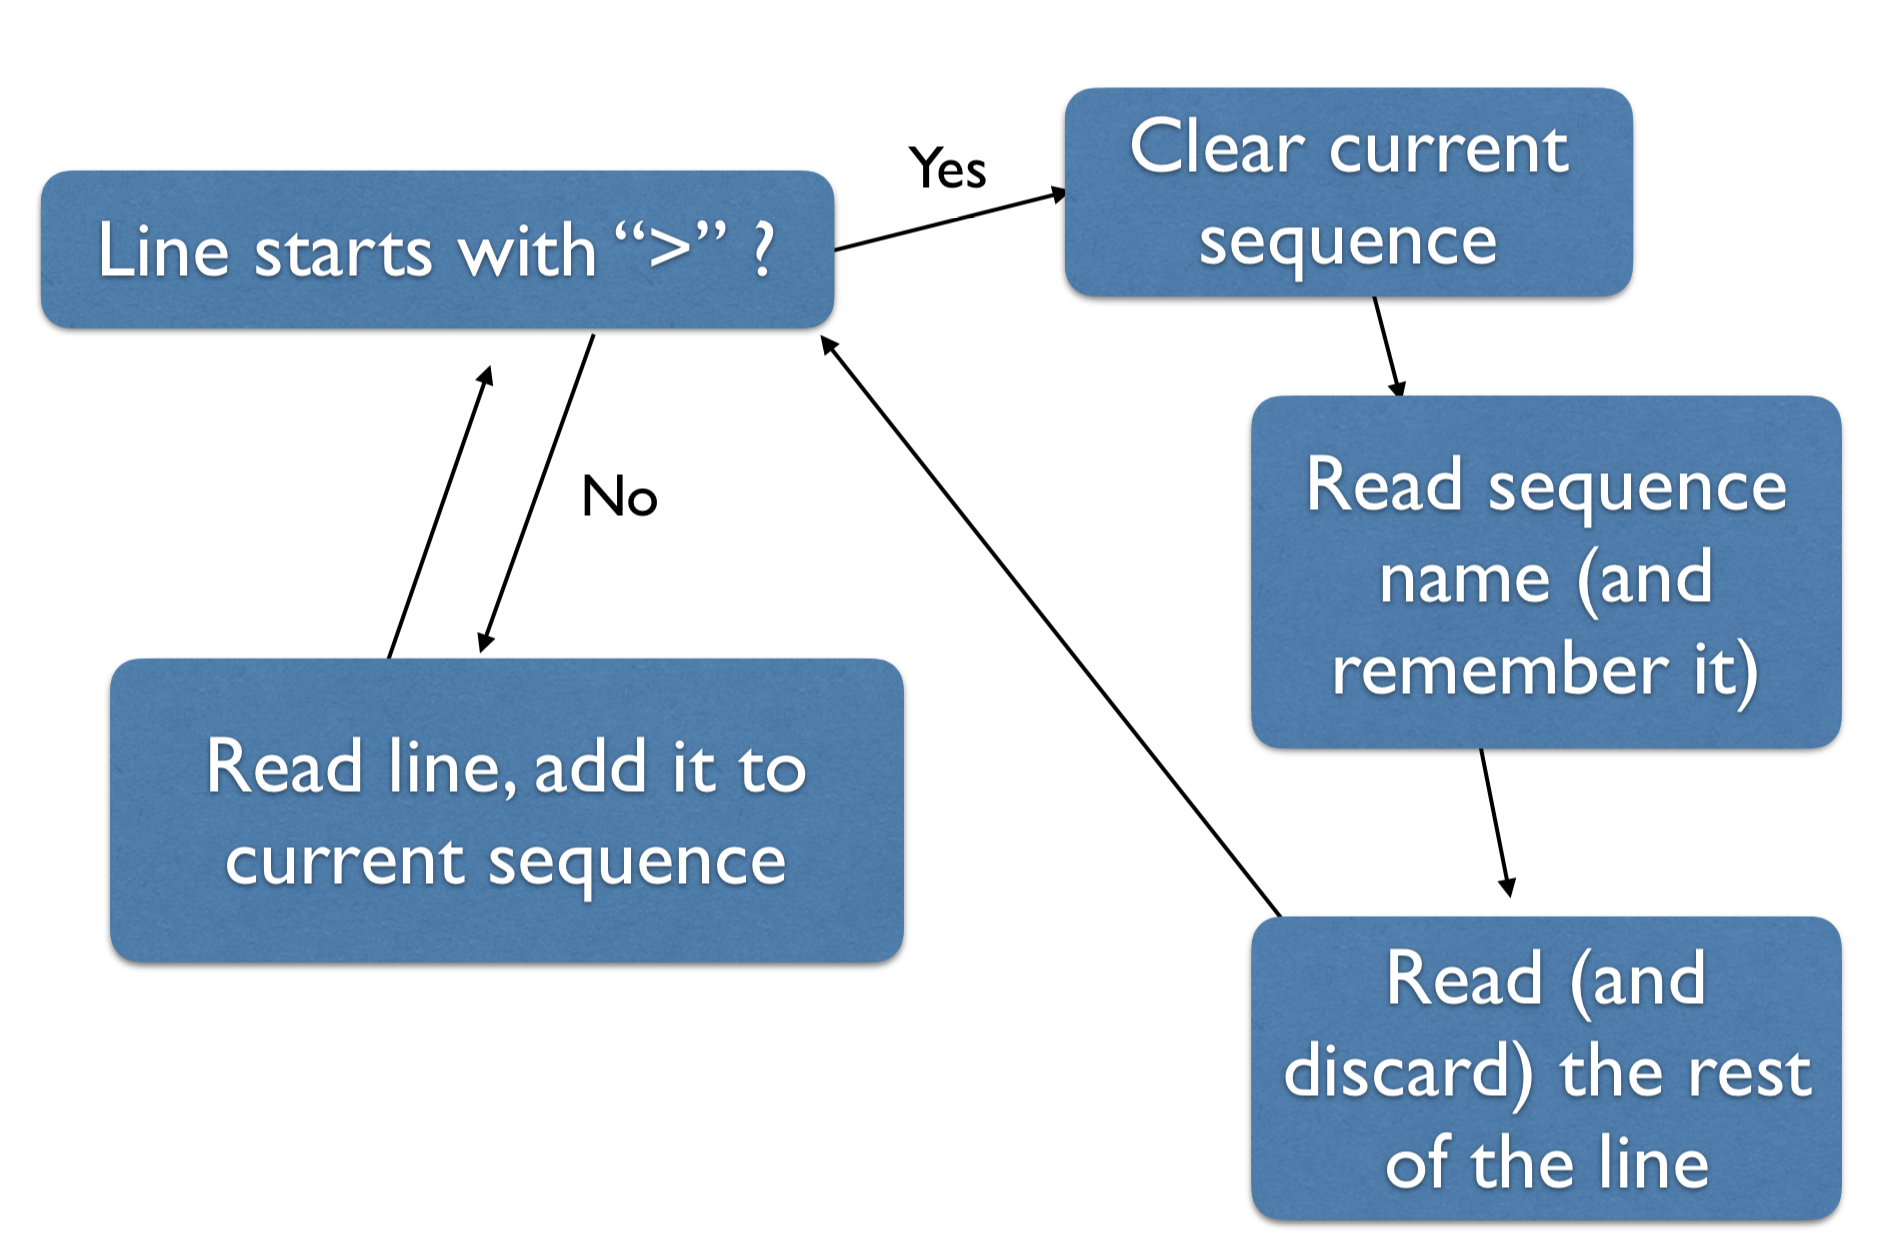
\includegraphics[width=.7\linewidth]{fasta_parse}
\end{figure}
   

\section{Summary}
File formats are very important in storing the diverse types of data used in computational biology. When thinking about each filetype, some important things considerations include how big the file is, what data is includes, what data does it exclude, and what is the goal of the format. Another important consideration is if the data is being stored {\it efficiently}. This includes how the format scales with data size, and how compression affects the quality of the data (lossless compression vs lossy compression). In summary, the right file format go a long way when conducting bioinformatic experiments!
\end{document}




